\documentclass[UTF8]{ctexart}

\title{杂谈勾股定理}
\author{张三}
\date{\today}
\bibliographystyle{plain} % 声明参考文献格式

% 插图功能的相关宏包
\documentclass{ctexart}
\usepackage{graphicx}

% 引用公式同时产生括号
\usepackage{amsmath}

% 在表格很小不影响分页,用这个包
\usepackage{float}
% 以上为导言区
\begin{document}

  \maketitle % 排版题目信息
  \begin{abstract}
    这是一篇关于勾股定理的文章
  \end{abstract}
  \tableofcontents % 命令输出目录
  \section{勾股定理在古代}
    勾股定理(英语Pythagorean theorem)又称商高定理(公元前 12 世纪)、毕达哥拉斯定理、毕氏定理、百牛定理,是平面几何中一个基本而重要的定 理。\cite{Kline}
    % 汉字左右的空格会被忽略

    % 使用空行分段,空行只有分段作用,段前不用打空格
    勾股定理说明,平面上的直角三角形的两条直角边的长度(古称勾长、股长)的平方和等于斜边长(古称弦长)的平方。反之,若平面上三角形中两边长的平方和等于第三边边长的平方,则它是
    % 换行相当于空格,只是分隔作用
    直角三角形(直角所对的边是第三边)。\cite{quanjing}
    % cite命令的参数是引用标签,也就是bib文件第一个出现的东西

    \begin{thm}[勾股定理]
      直角三角形斜边的平方等于两腰的平方和
    \end{thm}

    巴比伦人得到的勾股数的数量和质量不太可能纯从测量手段获得。之后的毕达哥拉斯本人并无著作传世,不过在他死后一千年,
    % 添加脚注
    5世纪的普罗克勒斯给欧几里德\footnote{欧几里德,约公元前330--275年}
    的名著《几何原本》做注解时将最早的发现和证明归功于毕达哥拉斯学派.

    在中国,记载秦朝的算数书并未记载勾股定理,只是记录了一些勾股数。定理首次载于书面则是在成书于西汉但内容收集整理自公元前一千多年以来的《周髀算经》“荣方问于陈子”一节中:
    \begin{quote}% 它将环境中的内容单独分行,增加缩进和上下间距,突出引用部分
    \zihao{-5}% 字号选择(-5 就是小五号)
    \kaishu% 使用楷书
      若求邪至日者,以日下为句,日高为股,句股各自乘,并而开方除之,得邪至日。

      --《周髀算经》卷上之二
    \end{quote}

  \section{数学公式}
    \subsection{行内公式(inline formula,或正文公式in-text formula)}
      $a+b$
    \subsection{列表公式}
      对于较长的公式或者比较重要的公式,单独给公式编号

      \begin{equation}\label{eq:gougu}
        \angle ACB = \pi /2

        AB^2 = BC^2 + AC^2
      \end{equation}

      勾股定理 \ref{eq:gougu} % 对公式的引用

      满足\eqref{eq:gougu}的整数称为\emph{勾股数}

      这样引用能可以产生括号,不过要加入宏包amsmath
    \subsection{上标下标}

      $2^{10} = 1024$

      $90^\circ$
  \section{使用图表}

      \subsection{插图}

        % figure 环境,就是插图使用的浮动体环境,相当于普通段落,没有缩进
        \begin{figure}[ht]% 可选参数ht表示可以出现在文字所在处(here)或顶部
          \centering% 后面内容居中
          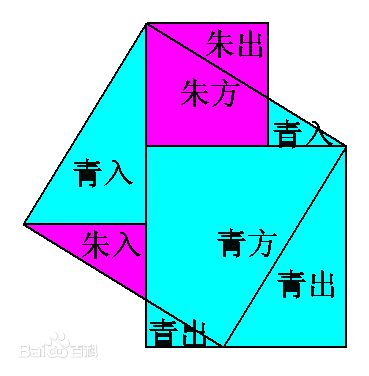
\includegraphics[width=3cm]{pythagorean_theorem.jpg}
          % \includegraphics有两个参数,方括号中的可选参数设定了宽度
          % 可选参数有[scale=放缩因子][height=高度][width=宽度]
          % 第二个参数是文件名,放在源文件目录
          \caption{青朱出入图}% 给插图加上编号和标题
          \labal{fig:qzcrt}
        \end{figure}
      青朱出入图\ref{fig:qzcrt},
      % 对图片标签的引用
      是东汉末年数学家刘徽根据“割补术”运用数形关系证明勾股定理的几何证明法,特色鲜明、通俗易懂。
      刘徽描述此图,“勾自乘为朱方,股自乘为青方,令出入相补,各从其类,因就其余不动也,合成弦方之幂。开方除之,即弦也。”其大意为,一个任意直角三角形,以勾宽作红色正方形即朱方,以股长作青色正方形即青方。将朱方、青方两个正方形对齐底边排列,再以盈补虚,分割线内不动,线外则“各从其类”,以合成弦的正方形即弦方,弦方开方即为弦长。 [3]
    \section{插入表格}
      下表列出了几个勾股数:
      \begin{table}[H]% 正文与表格连在一起就放在这里,不浮动,需要float包
        \begin{tabular}{|rrr|}%|rrr|表示有三列,都是右对齐
          \hline% 产生一条横线
          直角边$a$ & 直角边$b$ & 斜边$c$ \\% 项与项用\\隔开
          \hline
          3& 4& 5\\% 行与行用\\隔开
          5& 12& 13\\
          \hline
        \end{tabular}%
        % 上面的注释可以取消换行
        \qquad% 产生2em(约两个M宽)空白
        ($a^2 + b^2 = c^2$)
      \end{table}
  \nocite{Shiye}% 只在参考文献中显示,不直接引用
  \bibliography{math} % 提示从math数据库获取文献信息,来打印参考文献


\end{document}
